%%PREAMBLE %%%%%%%%%%%%%%%%%%%%%%%%%%%%
\documentclass[10pt, a4paper]{article}% size of txt = 10pt
\usepackage[top= 2cm,
			bottom = 2cm,
			left = 1.7cm,
			right = 1.7cm,
			footskip = 0.5cm,
			headsep = 0cm,
			headheight = 0cm
					]{geometry}
\usepackage{amsmath} % math packages
\usepackage{amsfonts}% math packages
\usepackage{amssymb} % math packages
\usepackage{graphicx} %package for including graphics
\usepackage{array}
\usepackage[thinlines]{easytable}
\usepackage{float}
\usepackage[section]{placeins}
\usepackage[hidelinks]{hyperref}
\usepackage[shortlabels]{enumitem}
\usepackage{svg}
\usepackage{bigstrut}
\usepackage{wrapfig,lipsum,booktabs}
\usepackage{subcaption}
\usepackage{xfrac}
\usepackage{pdfpages}
\usepackage{listings}
\usepackage{xcolor}


\usepackage{listings}
\usepackage{color} %red, green, blue, yellow, cyan, magenta, black, white
\definecolor{mygreen}{RGB}{28,172,0} % color values Red, Green, Blue
\definecolor{mylilas}{RGB}{170,55,241}

\definecolor{codegreen}{rgb}{0,0.6,0}
\definecolor{codegray}{rgb}{0.5,0.5,0.5}
\definecolor{codepurple}{rgb}{0.58,0,0.82}
\definecolor{backcolour}{rgb}{1,1,1}

\lstdefinestyle{mystyle}{
    backgroundcolor=\color{backcolour},   
    commentstyle=\color{codegreen},
    keywordstyle=\color{magenta},
    numberstyle=\tiny\color{codegray},
    stringstyle=\color{codepurple},
    basicstyle=\ttfamily\footnotesize,
    breakatwhitespace=false,         
    breaklines=true,                 
    captionpos=b,                    
    keepspaces=true,                 
    numbers=left,                    
    numbersep=5pt,                  
    showspaces=false,                
    showstringspaces=false,
    showtabs=false,                  
    tabsize=2
}
\lstset{style=mystyle}


%date format
\def\mydate{\leavevmode\hbox{\twodigits\day.\twodigits\month.\the\year}}
\def\twodigits#1{\ifnum#1<10 0\fi\the#1}

\usepackage{indentfirst}
\setlength{\parindent}{1cm}

\makeatletter
\newcommand{\thickhline}{%
    \noalign {\ifnum 0=`}\fi \hrule height 2pt
    \futurelet \reserved@a \@xhline
}
\newcolumntype{"}{@{\hskip\tabcolsep\vrule width 2pt\hskip\tabcolsep}}
\makeatother
\newcolumntype{?}{!{\vrule width 2pt}}
%%DOC ENVIROMENT%%%%%%%%%%%%%%%%%%%%%%%
\begin{document}
%Title 
\begin{flushleft}%% left justification
	\textbf{\Large{MKC-NBS: Úkol č. 1}}\hfill Filip Paul\\
	\large{Kryptografie \hfill\mydate}
\end{flushleft}
\section*{\large{\textbf{Bloková šifra v režimu CBC:}}}
	\begin{enumerate}
		\item \textbf{Zadání:}\\
			Mějme zprávu Z = (13, 4, 9), kde jednotlivá čísla jsou bloky zprávy. Tuto zprávu zašifrujte v režimu
			CBC pro inicializační vektor IV = 6. Vypočítaný kryptogram pro kontrolu dešifrujte. Šifrování E a
			dešifrování D je dáno substitucemi podle tabulky 1. K provedení operací XOR si dekadická čísla
			převeďte na čtyřbitová čísla. Pro daný provozní režim nakreslete diagramy podle první přednáškové
			prezentace (snímek č. 21), přičemž v datových blocích schématu uveďte dekadicky i binárně
			hodnotu příslušného vstupu, či výstupu.

			% Table generated by Excel2LaTeX from sheet 'List1'
			\begin{table}[htbp]
				\centering
				\caption{Šifrovací substituce y = E(x,K)}
				\begin{tabular}{?c?c|c|c|c|c|c|c|c|c|c|c|c|c|c|c|c?}
				\thickhline
				X  & 0  & 1  & 2  & 3  & 4  & 5  & 6  & 7  & 8  & 9  & 10 & 11 & 12 & 13 & 14 & 15 \bigstrut\\
				\thickhline
				Y  & 4  & 10 & 9  & 2  & 13 & 8  & 0  & 14 & 6  & 11 & 1  & 12 & 7  & 15 & 5  & 3 \bigstrut\\
				\thickhline
				\end{tabular}%
				\label{tab:sifrTab}%
			\end{table}%

		\item \textbf{Vypracování:}\\
		Na následujícím obrázku jsou vyznačeny stavy v decimální i binární podobě pro každý "stupeň"
		blokové šifry. Tyto hodnoty byly vypočítány pomocí python scriptu přiloženého na konci tohoto pdf souboru.
		Nicméně pro lepší zobrazení scriptu můžete využít link na můj github repozitář $\rightarrow$ 
		\href{https://github.com/FilipPaul/ctvrtak_letni_semestr/tree/main/MKC_NSB/ukol1_kryptografie}{\color{blue} PYTHON CBC.py}

		\begin{figure}[ht!]
			\centering
			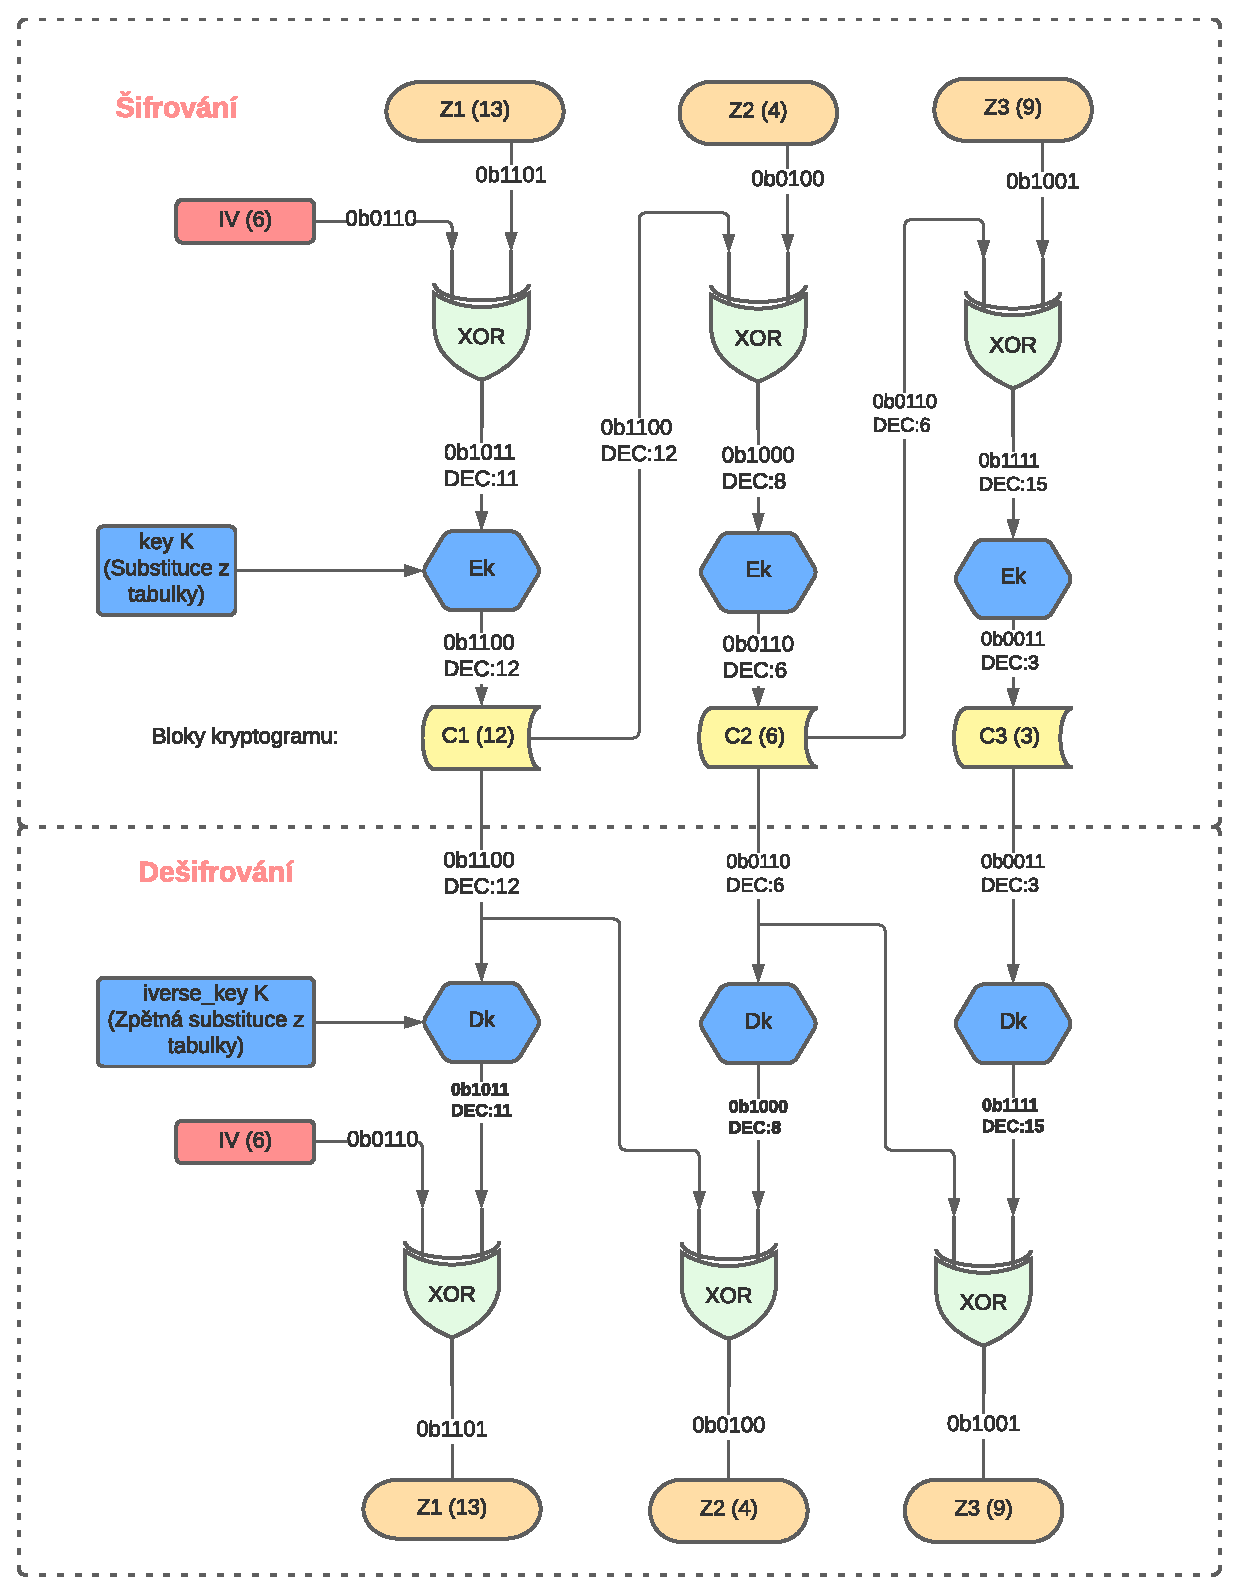
\includegraphics[width = 1\textwidth]{CBC_drawing.eps}
		\end{figure}
 	
	\end{enumerate}
\clearpage
	\section*{\large{\textbf{Výpočet pečeti HMAC}}}
		\begin{enumerate}
			\item \textbf{Zadání:}\\
				Mějme zprávu Z = (13, 4, 9), kde jednotlivá čísla jsou bloky zprávy. Pro tuto zprávu vypočítejte
				technikou HMAC pečeť P. Pečetící klíč K = 7, konstanta $C_1$ = 13 a $C_2$ = 8. K provedení operací
				XOR si dekadická čísla převeďte na čtyřbitová čísla. Hešovací funkce H je definována následovně:\\\\
				$h = \left( \sum_{i = 1}^{t}  a^i \cdot v_i \right) mod 17$\\\\
				kde hešovací konstanta a = 11, $v_i$ je i-tý blok hešovaného vstupu a t počet bloků na vstupu. V prvém
				hešování tedy bude t = 4, protože první blok je výsledek xorování klíče a konstanty a další bloky
				jsou bloky zprávy. Ve druhém hešování bude t = 2. Pečetí P je výstup z druhého hešování, tj. P = $h_2$.
				\item \textbf{Vypracování:}\\
				Podobně jako v předcházejícím úkolu byla úloha řešena pomocí python
				\href{https://github.com/FilipPaul/ctvrtak_letni_semestr/tree/main/MKC_NSB/ukol1_kryptografie}{\color{blue} scriptu}.
				Na následujícím obrázku jsou znázorněny jednotlivé "stavy" heshovací funkce HMAC v binární i decimální podobě.
				\begin{figure}[ht!]
					\centering
					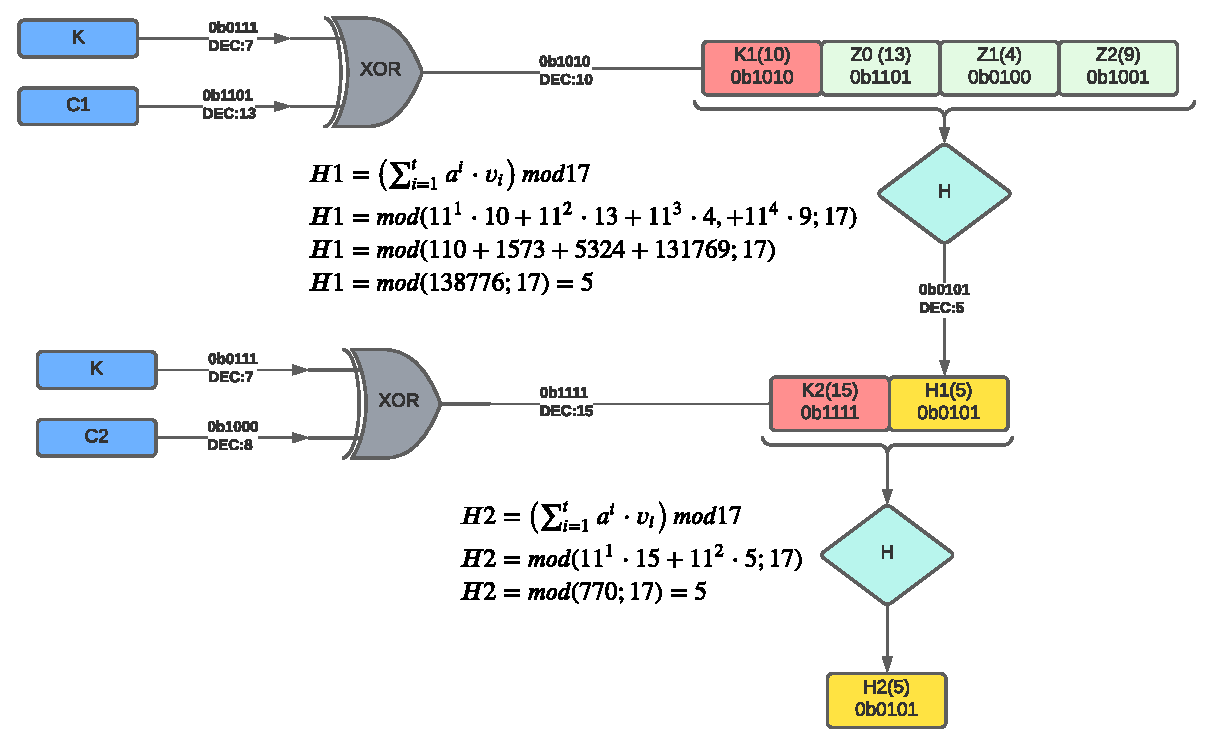
\includegraphics[width = 1\textwidth]{HMAC_drawing.eps}
				\end{figure}
		\end{enumerate}

		\section*{\large{\textbf{RSA podpis}}}
		\begin{enumerate}
			\item \textbf{Zadání:}\\
				Byla Vám doručena zpráva Z = (13, 4, 9), jejíž RSA podpis DS = 5. Ověřte, zda je tato zpráva
				autentická. Znáte veřejný ověřovací klíč udávaného autora VK = 3, jeho modulus n = 33 a víte, že
				byla použita hešovací funkce H ze 2. příkladu.
			\item \textbf{Vypracování:}\\

		\end{enumerate}
	\section*{\large{\textbf{Přiložené soubory}}}
	\lstinputlisting[language=python]{cbc.py}
	Output:\\
	xor\_1: init\_vect(DEC:6, BIN:0110) XOR Z\_0(DEC:13, BIN:1101)\\
	Encription\_input\_1: (DEC:11, BIN:1011)\\
	Cryptogram\_1: (DEC:12, BIN:1100)\\
	xor\_2: init\_vect(DEC:12, BIN:1100) XOR Z\_1(DEC:4, BIN:0100)\\
	Encription\_input\_2: (DEC:8, BIN:1000)\\
	Cryptogram\_2: (DEC:6, BIN:0110)\\
	xor\_3: init\_vect(DEC:6, BIN:0110) XOR Z\_2(DEC:9, BIN:1001)\\
	Encription\_input\_3: (DEC:15, BIN:1111)\\
	Cryptogram\_3: (DEC:3, BIN:0011)

\end{document}

%\[f(x)= (x+2)^2 - \frac{9\cdot 2\pi}{26}\] %%mathematic equatation in display style mode
%%optional:
%	\begin{align} %%this alignes all charakters after & if *is removed equations will be numbered
%	\hspace{5cm}  
%		 x &= a_2 x^2 +_1 x + a_0 \\
% 		x &=x^2 \nonumber		%no number will not add number to eq
%	\end{align}